\label{sec:Anwendungsszenarien}

Im Folgenden werden Anwendungsszenarien für die \gls{CROP} dargestellt. Dabei
wird die Funktionsweise sowohl anhand eines Textes als auch eines Bildes beschrieben und
verglichen. Dies erfolgt von der Eingabe über die Splittung bis hin zum Versand
der Nachricht.

Die Art und Weise wie ein Bild oder ein Text untersucht und bearbeitet wird
unterscheidet sich. Im Rahmen dieser Arbeit wird ein Text als
Anwendungsszenario herangezogen. Grundlage bildet hierbei eine Nachricht,
welche der Nutzer über eine grafische Benutzeroberfläche eingibt.
Dabei ist zusätzlich ein manuelles Hervorheben der wichtigen Textpassagen
notwendig. Zur näheren Erläuterung soll folgendes fiktives Testszenario zur
Betrachtung herangezogen werden:

\textit{\glqq Gestern um 8 Uhr Marszeit wurden Hinweise auf mögliches Leben auf
dem Mars entdeckt, wobei ein Mann schwer verletzt wurde! \grqq}

Für unser Szenario haben wir aus Testgründen folgende Relevanzsetzungen
festgelegt. Die höchste Aufmerksamkeit gilt der Tatsache, dass mögliches Leben
entdeckt und dabei ein Mann schwer verletzt wurde. Demnach bekommen diese beiden
Abschnitte die höchste Priorität. Folgen könnte die Uhrzeit, damit der Empfänger
zuordnen kann, wie lange die Verletzung bereits vorliegt. Alle weiteren Wörter
stellen zusätzliche Daten dar, die für die Vollständigkeit des Textes, aber
nicht zum Verständnis der Situation notwendig sind. Die Abbildung
\ref{fig:prioChatWindow} zeigt die Prioritäten in der ChatGui, auf die im
Kapitel \ref{cap:chatGui} noch näher eingegangen wird.

\begin{figure}[H]
	\centering
	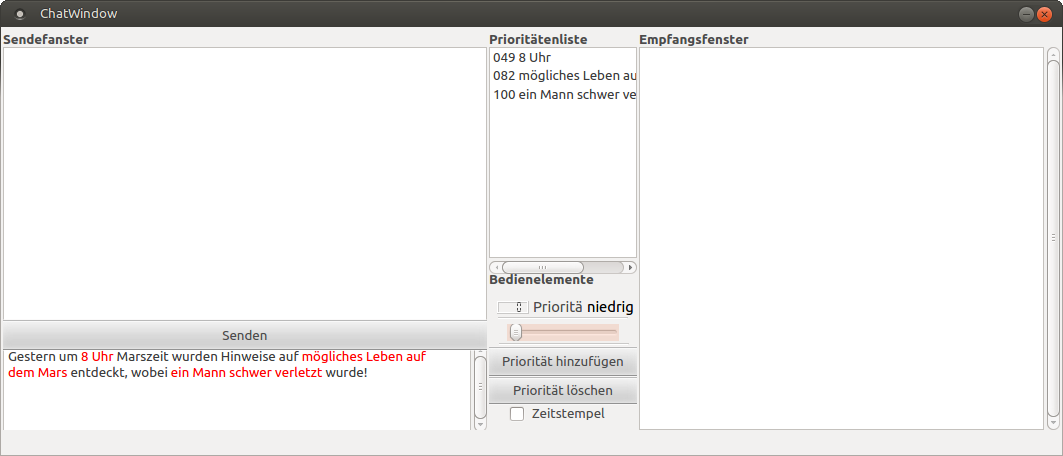
\includegraphics[width=\textwidth]{prioChatWindow.png}
	\label{fig:prioChatWindow}
	\caption{Chat-Fenster mit priorisierter Eingabe}
\end{figure}

Der Text wird jetzt Wort für Wort untersucht und anhand der Priorität sortiert.
Dabei bilden Wortgruppen mit gleicher Relevanz einen Datenblock, dem eine
Sequenznummer zugeordnet wird, wodurch eine eindeutige Identifizierung möglich
ist. Die \gls{DOID} beugt einer Verwechslung anderer Datenblöcke gleicher
Sequenznummer vor. Weiterhin werden die Position und die Länge der Wortgruppe im
Text abgespeichert. Anhand dieser Informationen ist der Empfänger in der Lage,
die ankommenden Datenblöcke korrekt zuzuordnen und so den Text
wiederherzustellen.
In Abbildung \ref{fig:chatguiexample} ist dargestellt, wie einzelne Fragmente
zuerst ankommen und der Text mit jedem weiteren Datenpaket vervollständigt wird.

\begin{figure}[H]
	\centering
	\subfigure{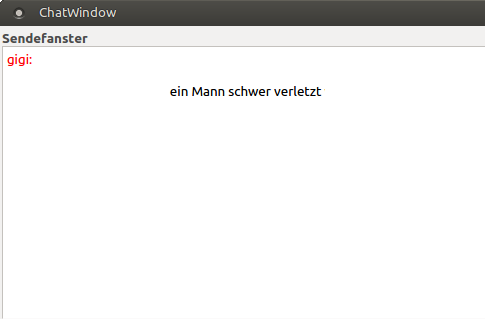
\includegraphics[scale=.6]{chatGuiWindow_empfaenger_prio.png}}\\
	\subfigure{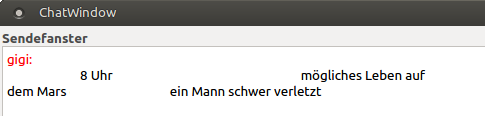
\includegraphics[scale=.6]{chatGuiWindow_empfaenger_halfPrio.png}}\\
	\subfigure{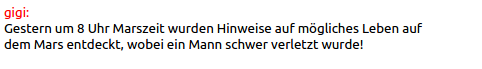
\includegraphics[scale=.6]{chatGuiWindow_empfaenger_all.png}}
	\label{fig:chatguiexample}
	\caption{Wiederherstellung der Nachricht beim Empfänger}
\end{figure}

Bei der Übertragung von Bildern (derzeit nicht implementiert) gestaltet sich der
grundsätzliche Ablauf ähnlich. Die Abbildung \ref{fig:marsWaterResidue} (a)
zeigt das vom Marsrover \textit{Curiosity} am $28.$ September aufgenommene
ausgetrocknete Wasserbett. Der im linken Bild markierte Bereich zeigt,
Wissenschaftlern zufolge, einen vom Wasser verformten Kiesel \cite{web11}. Wie
beim Szenario zuvor erfolgt zunächst eine Markierung der wichtigen Bereiche.
Diese sind der Kiesel und der Maßstab, welche in der Abbildung
\ref{fig:marsWaterResidue} (b) dargestellt werden. Bevor das Bild Schritt für
Schritt analysiert wird, muss dieses in Abschnitte eingeteilt werden, welche
später die einzelnen Datenblöcke darstellen.
 
\begin{figure}[H]
	\centering
	\subfigure[Originalbild]{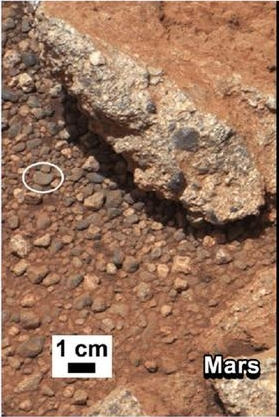
\includegraphics[scale=.4]{marsWaterResidue_links.jpg}}\hfill
	\subfigure[Markierung der Relevanz]
	 {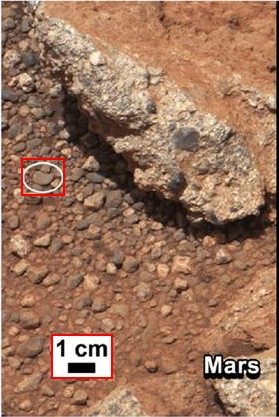
\includegraphics[scale=.4]{marsWaterResidue_mitte.jpg}}\hfill
	\subfigure[Zerlegung des Bildes]
	 {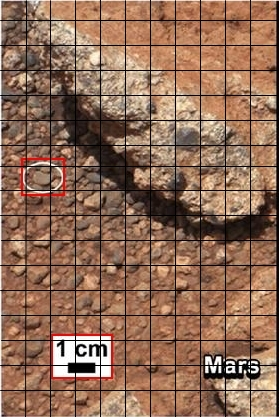
\includegraphics[scale=.4]{marsWaterResidue_rechts.jpg}}
	\label{fig:marsWaterResidue}
	\caption[Priorisierung des Bildes]{Priorisierung des Bildes \cite{img3}}
\end{figure}

Die weiteren Schritte sind äquivalent zu denen des Textes. Die beiden wichtigen
und damit höher priorisierten Bereiche erreichen den Empfänger zuerst.
Das Zusammensetzen des Bildes wird in seiner prinzipiellen Form in
Abbildung \ref{fig:marsWaterResidueEmpfaenger} dargestellt.

\begin{figure}[H]
	\centering
	\subfigure[leeres Bild]
	 {
\includegraphics[scale=.4]{marsWaterResidue_empfaenger_links.jpg}}\hfill
	\subfigure[empfangene wichtige Bereiche]
	 {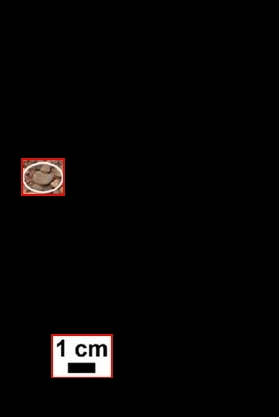
\includegraphics[scale=.4]{marsWaterResidue_empfaenger_mitte.jpg}}\hfill
	\subfigure[wieder zusammengesetztes Bild]
	 {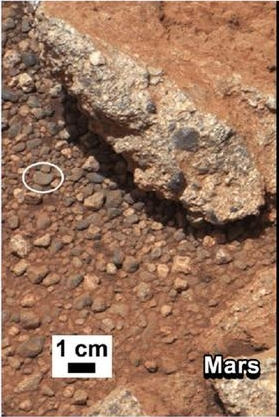
\includegraphics[scale=.4]{marsWaterResidue_empfaenger_rechts.jpg}}
	\label{fig:marsWaterResidueEmpfaenger}
	\caption{Wiederherstellung des Bildes}
\end{figure}